\documentclass[hide notes,intlimits]{beamer}

\mode<presentation>
{
  \usetheme[footline]{PISMshade}
  \setbeamercovered{transparent}
}

% load packages
\usepackage{multimedia}
\usepackage[english]{babel}
\usepackage[latin1]{inputenc}
\usepackage[T1]{fontenc}
\usepackage[multidot]{grffile}

\usepackage{tikz}
\usetikzlibrary{shapes,arrows}
\usetikzlibrary{shadows}

\definecolor{dark red}{HTML}{E41A1C}
\definecolor{dark green}{HTML}{4DAF4A}
\definecolor{dark violet}{HTML}{984EA3}
\definecolor{dark blue}{HTML}{084594}
\definecolor{dark orange}{HTML}{FF7F00}
\definecolor{light blue}{HTML}{377EB8}
\definecolor{light red}{HTML}{FB9A99}
\definecolor{light violet}{HTML}{CAB2D6}

\setbeamercolor{boxed}{fg=black,bg=light blue!25}
\graphicspath{{../figures_2018_08/}{../figures/}}

\newenvironment{transbox}[1][]{%
\begin{tikzpicture}
\node[drop shadow,rounded corners,text width=.9\textwidth,fill=white, fill opacity=#1,text opacity=1] \bgroup
}{
\egroup;\end{tikzpicture}} 

\newenvironment{transbox-tight}{%
\begin{tikzpicture}
\node[drop shadow,rounded corners,fill=uaf yellow, fill opacity=0.75,text opacity=1] \bgroup
}{
\egroup;\end{tikzpicture}} 

\newcommand{\jl}{[\![}
\newcommand{\jr}{]\!\hskip 0.003cm ]}
\newcommand{\bpsi}{\boldsymbol{\psi}}
\newcommand{\bPsi}{\boldsymbol{\Psi}}
\newcommand{\bphi}{\boldsymbol{\phi}}
\newcommand{\bPhi}{\boldsymbol{\Phi}}
\newcommand{\bn}{\mathbf{n}}
\newcommand{\bq}{\mathbf{q}}
\newcommand{\bv}{\mathbf{v}}
\newcommand{\D}{\,\mathrm{d}}
\newcommand{\Tsnow}{T_{\text{snow}}}
\newcommand{\Hatm}{H_{\text l}^{\text{atm}}}

\newcommand{\mathtext}[1]{\mathsf{#1}}

% title page
\title[Ice sheet modeling] % (optional, use only with long paper titles)
{Makming Greenland Green Again}

\author[Aschwanden] % (optional, use only with lots of authors)
{Many \& Andy Aschwanden}
% - Give the names in the same order as the appear in the paper.
% - Use the \inst{?} command only if the authors have different
%   affiliation.

% - Use the \inst command only if there are several affiliations.
% - Keep it simple, no one is interested in your street address.

\titlegraphic{\vskip-1.cm\includegraphics[height=4.5cm]{gris-green-again}}

\date{}


\subject{The Greenland Ice Sheet}

\begin{document}


\setbeamertemplate{background canvas}
  {
     \tikz{\node[inner sep=0pt,opacity=1.0] {\includegraphics[width=\paperwidth]{uaf_beamer_shade_bg}};}
} 

% insert titlepage
\begin{frame}
  \titlepage
  \note[item]{Collaboration between most glaciology faculty here at UAF}
  \note[item]{Mark F., Martin T., Regine H., and my former student Doug B.}
\end{frame}


\setbeamertemplate{background canvas}
  {
     \tikz{\node[inner sep=0pt,opacity=1] {\includegraphics[height=\paperheight,width=\paperwidth]{gris-green-collage-clean}};}
} 

\begin{frame}[plain]
  \note[item]{We know Greenland was nearly ice-free for extended periods during the Pleistocene}
  \note[item]{that's from 2.6 million years ago to 11,700 years ago}
  \note[item]{Maybe Greenland looked somehting like this}
\end{frame}

\setbeamertemplate{background canvas}
  {
     \tikz{\node[inner sep=0pt,opacity=1] {\includegraphics[height=\paperheight,width=\paperwidth]{gris-green-collage-1}};}
} 

\begin{frame}[plain]
  \note[item]{Lots of space to go hiking}
\end{frame}

\setbeamertemplate{background canvas}
  {
     \tikz{\node[inner sep=0pt,opacity=1] {\includegraphics[height=\paperheight,width=\paperwidth]{gris-green-collage-2}};}
} 

\begin{frame}[plain]
  \note[item]{For caribous to roam}
\end{frame}

\setbeamertemplate{background canvas}
  {
     \tikz{\node[inner sep=0pt,opacity=1] {\includegraphics[height=\paperheight,width=\paperwidth]{gris-green-collage-3}};}
} 

\begin{frame}[plain]
  \note[item]{or like a Jurassic Park}
  \note[item]{Now the intersting question is:}
  \note[item]{Can this happen again}
  \note[item]{and under what conditions?}

\end{frame}


\setbeamertemplate{background canvas}
{
%
}


\begin{frame}{Observed vs simulated flow speeds in 1999}
  \begin{columns}[c]
    \begin{column}{.65\linewidth}
    \begin{figure}
      \includegraphics[width=\textwidth]{gris-obs-exp-old-1999}
    \end{figure}
    \end{column}
    \begin{column}{.35\linewidth}
      \begin{figure}
        \includegraphics[width=\textwidth]{roadblocks}
      \end{figure}
      \begin{itemize}
      \item can't reproduce flow field
      \end{itemize}
    \end{column}
  \end{columns}
  \note[item]{}
\end{frame}

\begin{frame}{Observed vs simulated flow speeds in 2013}
  \begin{columns}[c]
    \begin{column}{.65\linewidth}
    \begin{figure}
      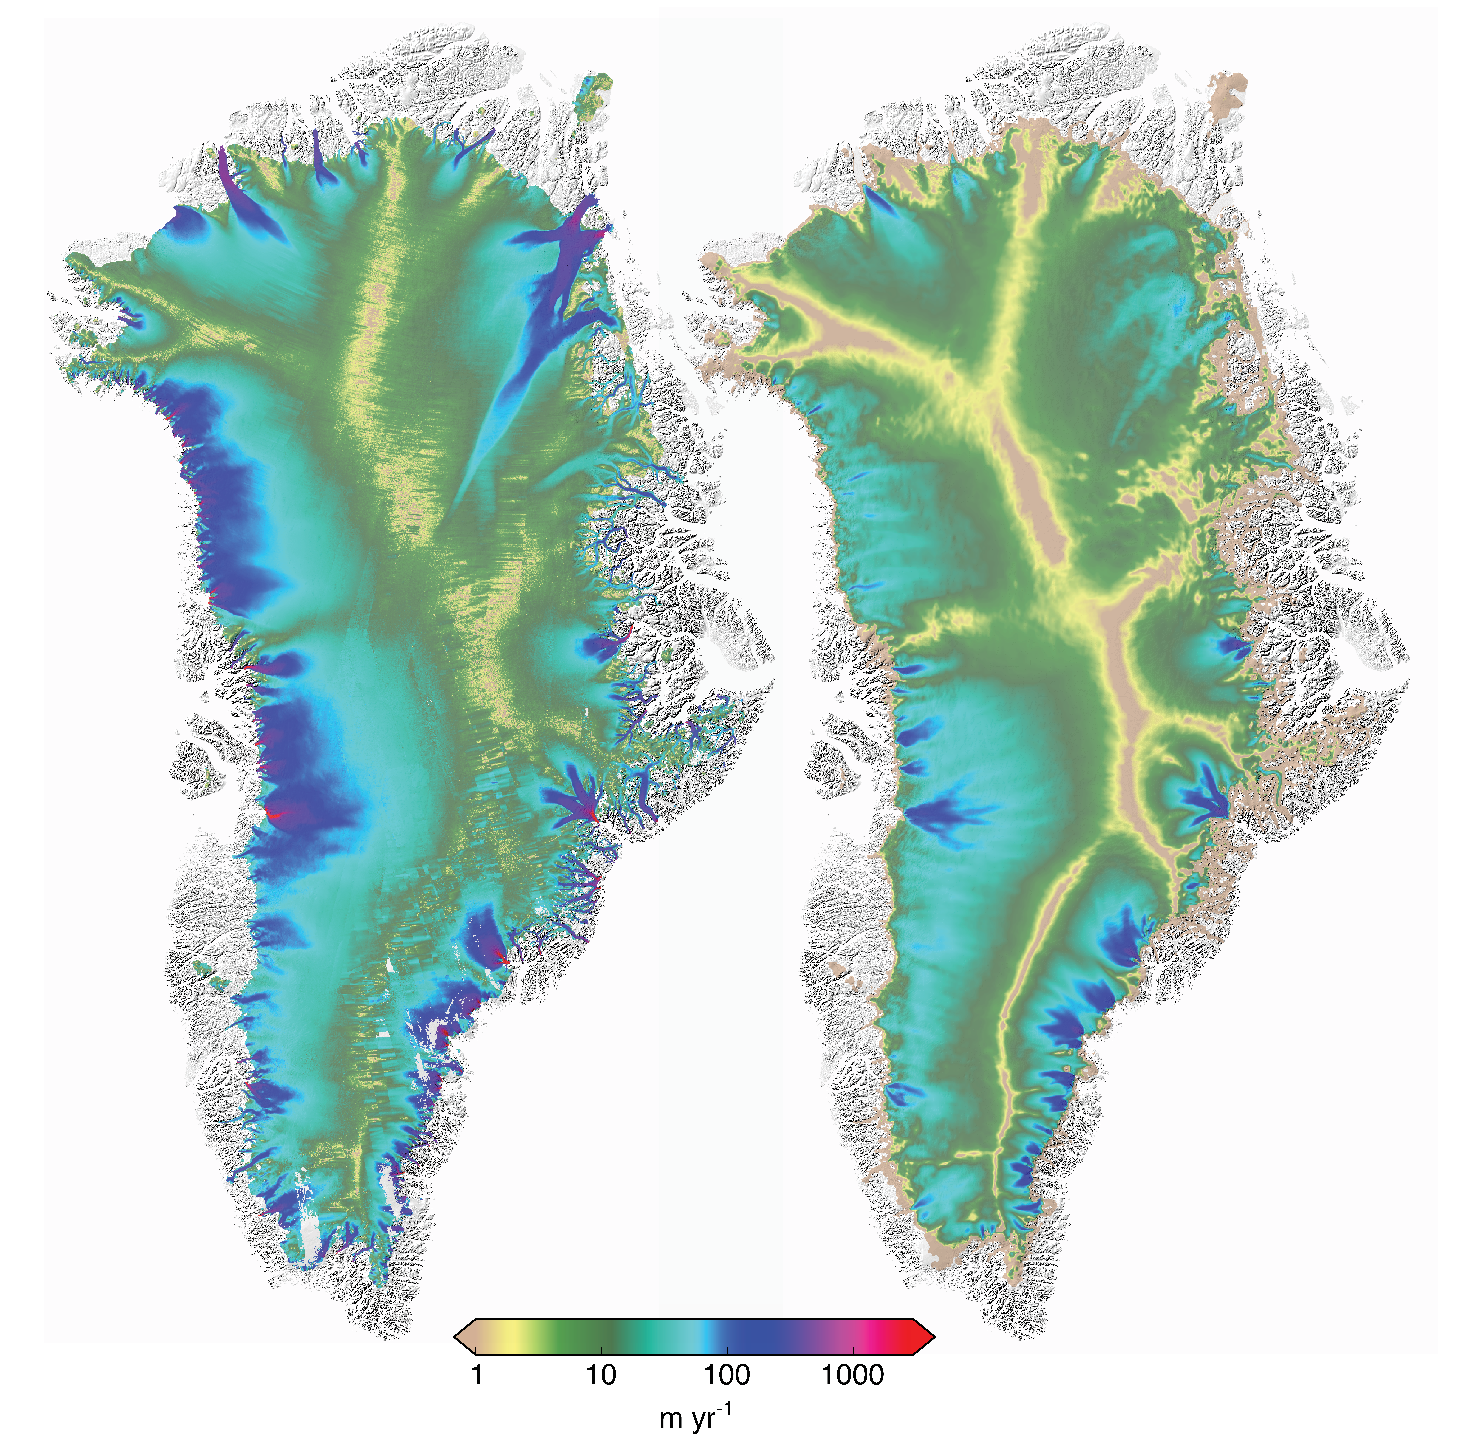
\includegraphics[width=\textwidth]{gris-obs-exp-old}
    \end{figure}
    \end{column}
    \begin{column}{.35\linewidth}
      \begin{figure}
        \includegraphics[width=\textwidth]{roadblocks}
      \end{figure}
      \begin{itemize}
      \item a bit better than in 1999
      \item but still can't reproduce flow field
      \end{itemize}
    \end{column}
  \end{columns}
  \note[item]{}
\end{frame}


\begin{frame}{Ice thickness and simulated flow speeds}
\vspace{-0.74em}
  \begin{columns}
    \column[c]{5cm}
    \begin{figure}
      \includegraphics<1-2>[width=\textwidth]{greenland-obs-basal-overview}
      \includegraphics<3-4>[width=\textwidth]{greenland-obs-basal-overview-mo14}
    \end{figure}
    \column[c]{5cm}
    \only<1,3>{Jakobshavn Isbr{\ae}}
    \only<2>{no fast flow}
    \only<4>{fast flow appears}
    \includegraphics<1>[width=\textwidth]{jakobshavn-bed-5000m-ba01}
    \includegraphics<2>[width=\textwidth]{jakobshavn-speed-exp-4500m-ba01}
    \includegraphics<3>[width=\textwidth]{jakobshavn-bed-mo14}
    \includegraphics<4>[width=\textwidth]{jakobshavn-speed-exp-600-v1.2-no-scale-no-gate}
    \only<1>{\\ 5\,km, old data set (2001)}
    \only<2,4>{\\ simulated surface speed}
    \only<3>{\\ 600\,m, new data set (2014)}
  \end{columns}
  \note<1>[item]{now let's do a simualulation with the old ice thickness data}
  \note<2>[item]{there isn't really any fast flow}
  \note<3>[item]{now use the new ice thickness}
  \note<4>[item]{and we get fast flow}
\end{frame}


\begin{frame}{We can capture the present-day flow field}
  \begin{figure}
    \includegraphics[height=7cm]{greenland-overview-3}
    \\ \scriptsize{Aschwanden, Fahnestock, Truffer (2016) \textit{Nature Communications}}
  \end{figure}
  \note[item]{first time capturing the flow field for the right reason}
  \note[item]{this is quite a break through in ice sheet modeling}
  \note[item]{though not a surprising one}
  \note[item]{it just confirms what students learn in glaciology 100:}
  \note[item]{ice flows downhill}
\end{frame}

\begin{frame}{Ready for a new assessment}
  \begin{figure}
    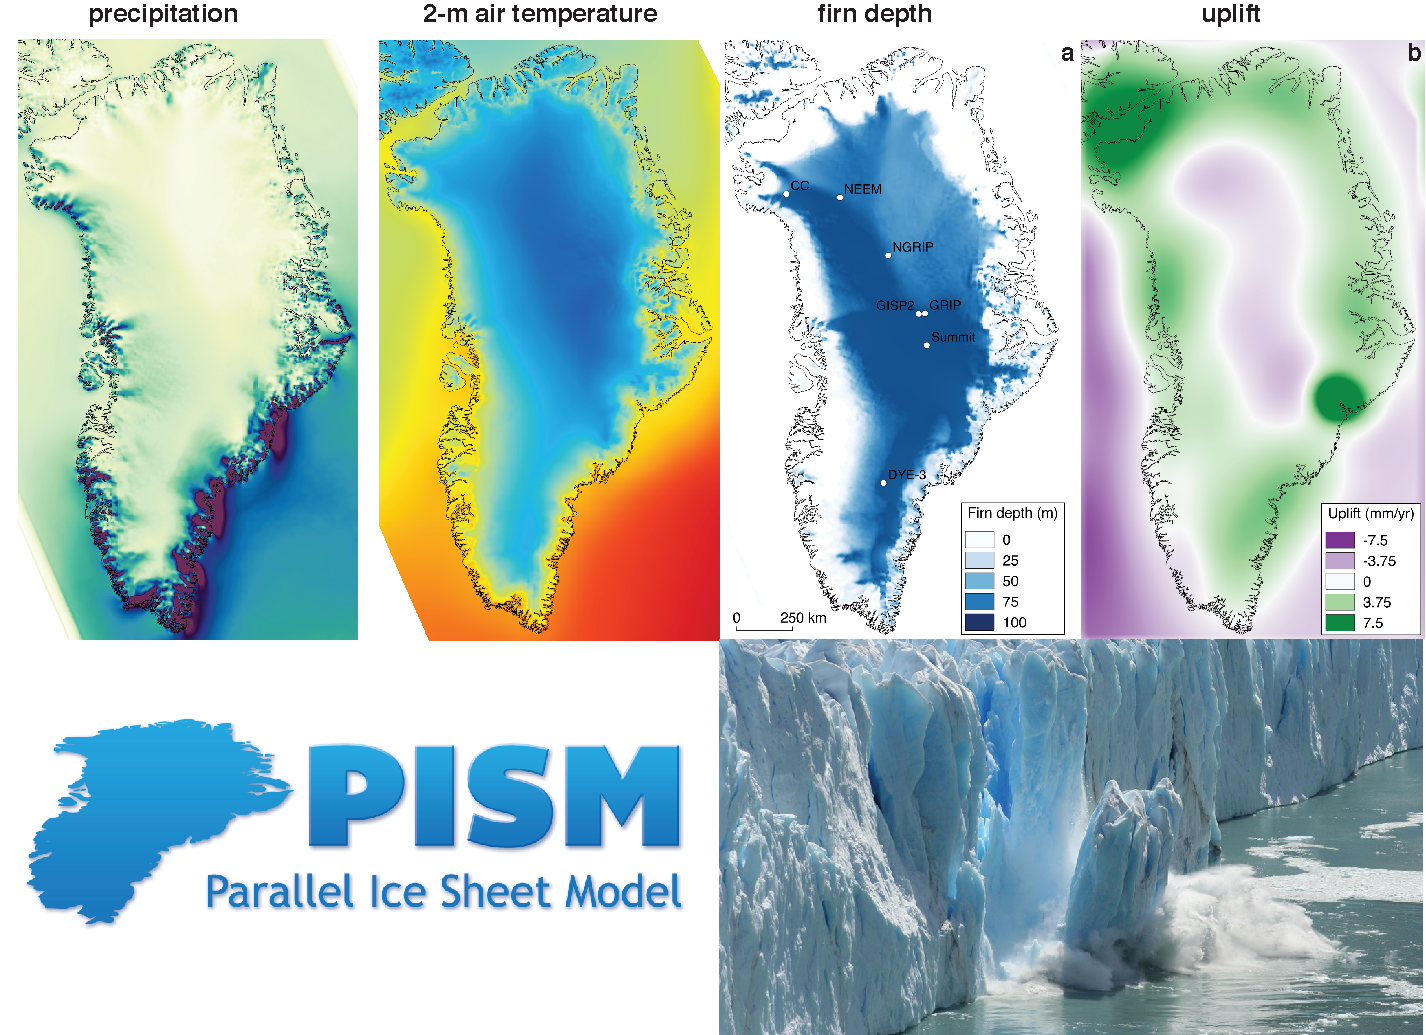
\includegraphics[width=11cm]{gris-pism-setup-2018}
  \end{figure}
  \note[item]{Over the past year, we've assembled the best data sets}
  \note[item]{added new model physics such better calving parameterizations}
  \note[item]{don't look at the figures carefully}
  \note[item]{to bring you the first post-AR5 sea level estimates}
  \note[item]{for the next millennium}
\end{frame}

\begin{frame}
  \frametitle{Evolution over the next millennium}
  \begin{columns}[c]
    \begin{column}{.85\linewidth}
    \begin{figure}
    \includegraphics[width=\textwidth]{les18_ctrl}
    \end{figure}
    \end{column}
    \begin{column}{.15\linewidth}
      \begin{figure}
        \includegraphics[height=1cm]{legend-rcp}
      \end{figure}
    \end{column}
  \end{columns}
\end{frame}


\begin{frame}
  \frametitle{Uncertainty analysis}
  \begin{columns}[c]
    \begin{column}{.3\linewidth}
    \begin{figure}
    \includegraphics[width=\textwidth]{parameter_histograms}
    \end{figure}
    \end{column}
    \begin{column}{.7\linewidth}
  \begin{itemize}
  \item choose the 4 GCMs and 10 parameters
  \item prescribe distributions (normal, uniform, truncated normal, gamma)
  \item draw 500 samples using Latin Hypercube Sampling
  \item run 500 simulations at 1.8\,km resolution per RCP (1,500 total)
  \item run control simulation at 900\,m resolution (ensemble mean forcing)
  \item Sobel indices attribution analysis
  \item 2M CPU hours
  \end{itemize}
    \end{column}
  \end{columns}
\end{frame}

\begin{frame}
  \frametitle{Evolution over the next millennium}
  \begin{columns}[c]
    \begin{column}{.85\linewidth}
    \begin{figure}
    \includegraphics[width=\textwidth]{les18_les}
    \end{figure}
    \end{column}
    \begin{column}{.15\linewidth}
      \begin{figure}
        \includegraphics[height=1cm]{legend-rcp}
      \end{figure}
    \end{column}
  \end{columns}
\end{frame}

\begin{frame}
  \frametitle{In a thousand years}
  \begin{figure}
    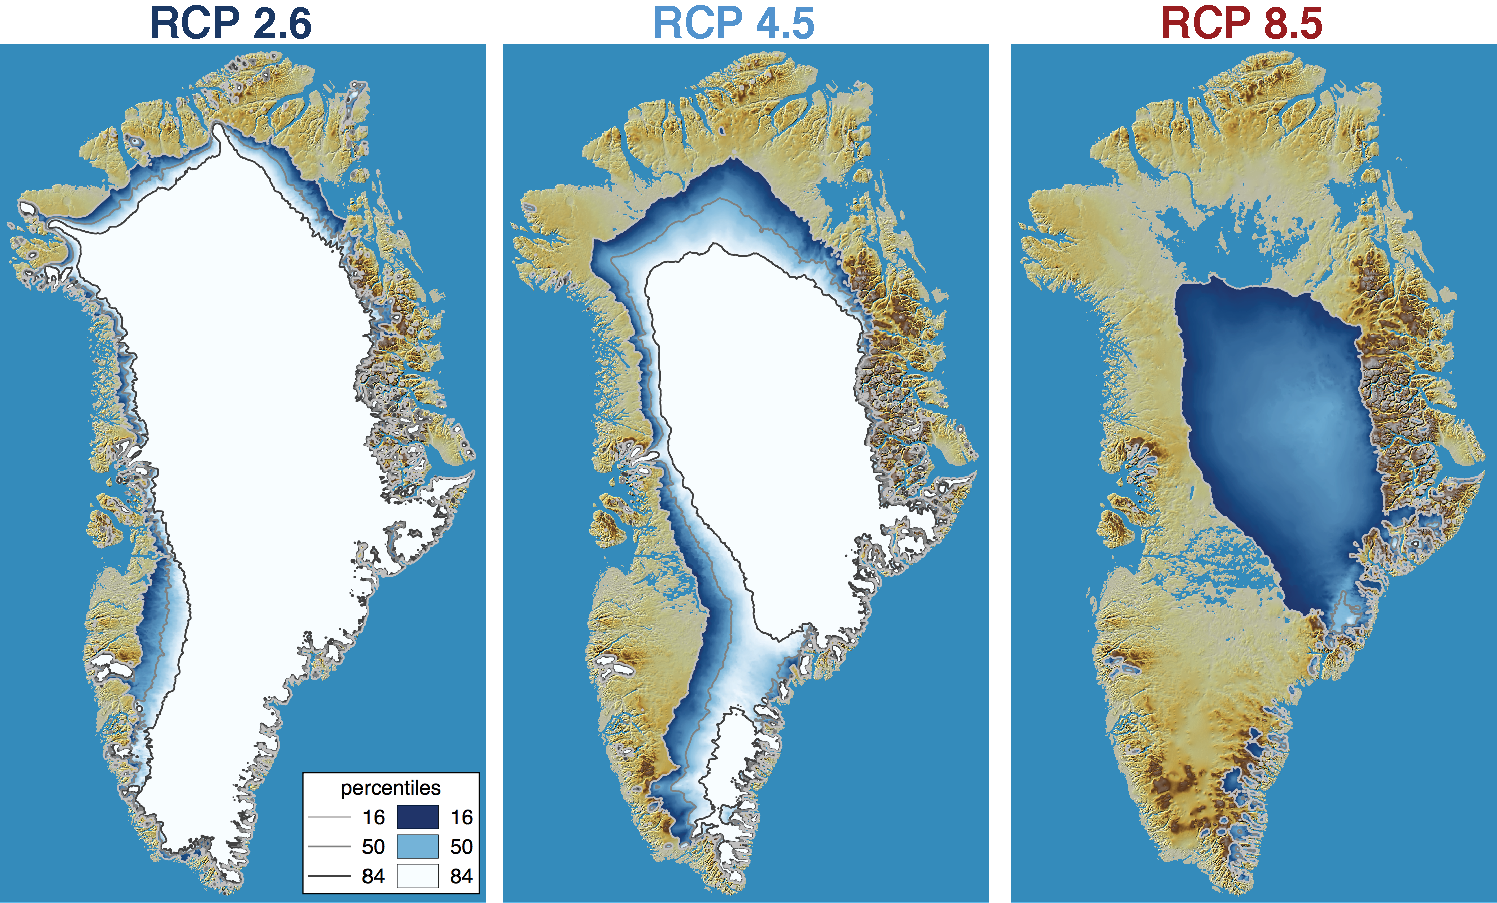
\includegraphics[height=6.5cm]{rcp-final-states-extend}
  \caption{Likelihood of a pixel being ice covered.}
  \end{figure}
  \note[item]{In a thousand years, Greenland will look different to today}
  \note[item]{Explain uncertainty map}

\end{frame}

\begin{frame}[plain]
  \begin{figure}
   \movie[showcontrols=true,autostart,loop,width=8cm]{\includegraphics[width=8cm]{../movies/gris_g900m_rcps_0000}}{../movies/gris-g900m_rcps-hd1920.mov}
  \end{figure}
\end{frame}


\begin{frame}
  \frametitle{Outlet glacier retreat}
  \begin{figure}
    \includegraphics<1>[width=\textwidth]{flowline-composite-1gl-uis} 
    \includegraphics<2>[width=\textwidth]{flowline-composite-1gl-sg} 
  \end{figure}
\end{frame}




\setbeamertemplate{background canvas}
  {
     \tikz{\node[inner sep=0pt,opacity=0.5] {\includegraphics[height=\paperheight,width=\paperwidth]{gris-green-collage-clean-50op}};}
} 

\begin{frame}
  \frametitle{Main Findings}
  \begin{transbox}
  \alert{$\Rightarrow$} Greenland could lose
  \begin{itemize}
    \item  5--19\,cm SLE (RCP 2.6), 8--23\,cm SLE (RCP 4.5), and 14--34\,cm SLE (RCP 8.5) by 2100
    \item  11--37\,cm SLE (RCP 2.6), 20--57\,cm SLE (RCP 4.5), and 52--156\,cm SLE (RCP 8.5) by 2200
  \end{itemize}
  \alert{$\Rightarrow$} Outlet glaciers will contribute
  \begin{itemize}
  \item 19--40\% of the total mass loss
  \end{itemize}
\end{transbox}
\end{frame}

\begin{frame}
  \frametitle{Main Findings}
  \begin{transbox}
    \begin{itemize}
    \item We have performed the first millennium scale projections with an \textbf{outlet glacier-resolving} ice sheet model 
    \item Greenland will very likely become ice free in a millennium if we stay on an RCP 8.5 path
      \item better characterization of basal and surface processes are needed
    \end{itemize}
  \end{transbox}
  \note[item]{In summary, Greenland will very likely become ice free within a millennium }
  \note[item]{if we keep following the RCP 8.5 scenario}
\end{frame}

\setbeamertemplate{background canvas}
  {
     \tikz{\node[inner sep=0pt,opacity=1] {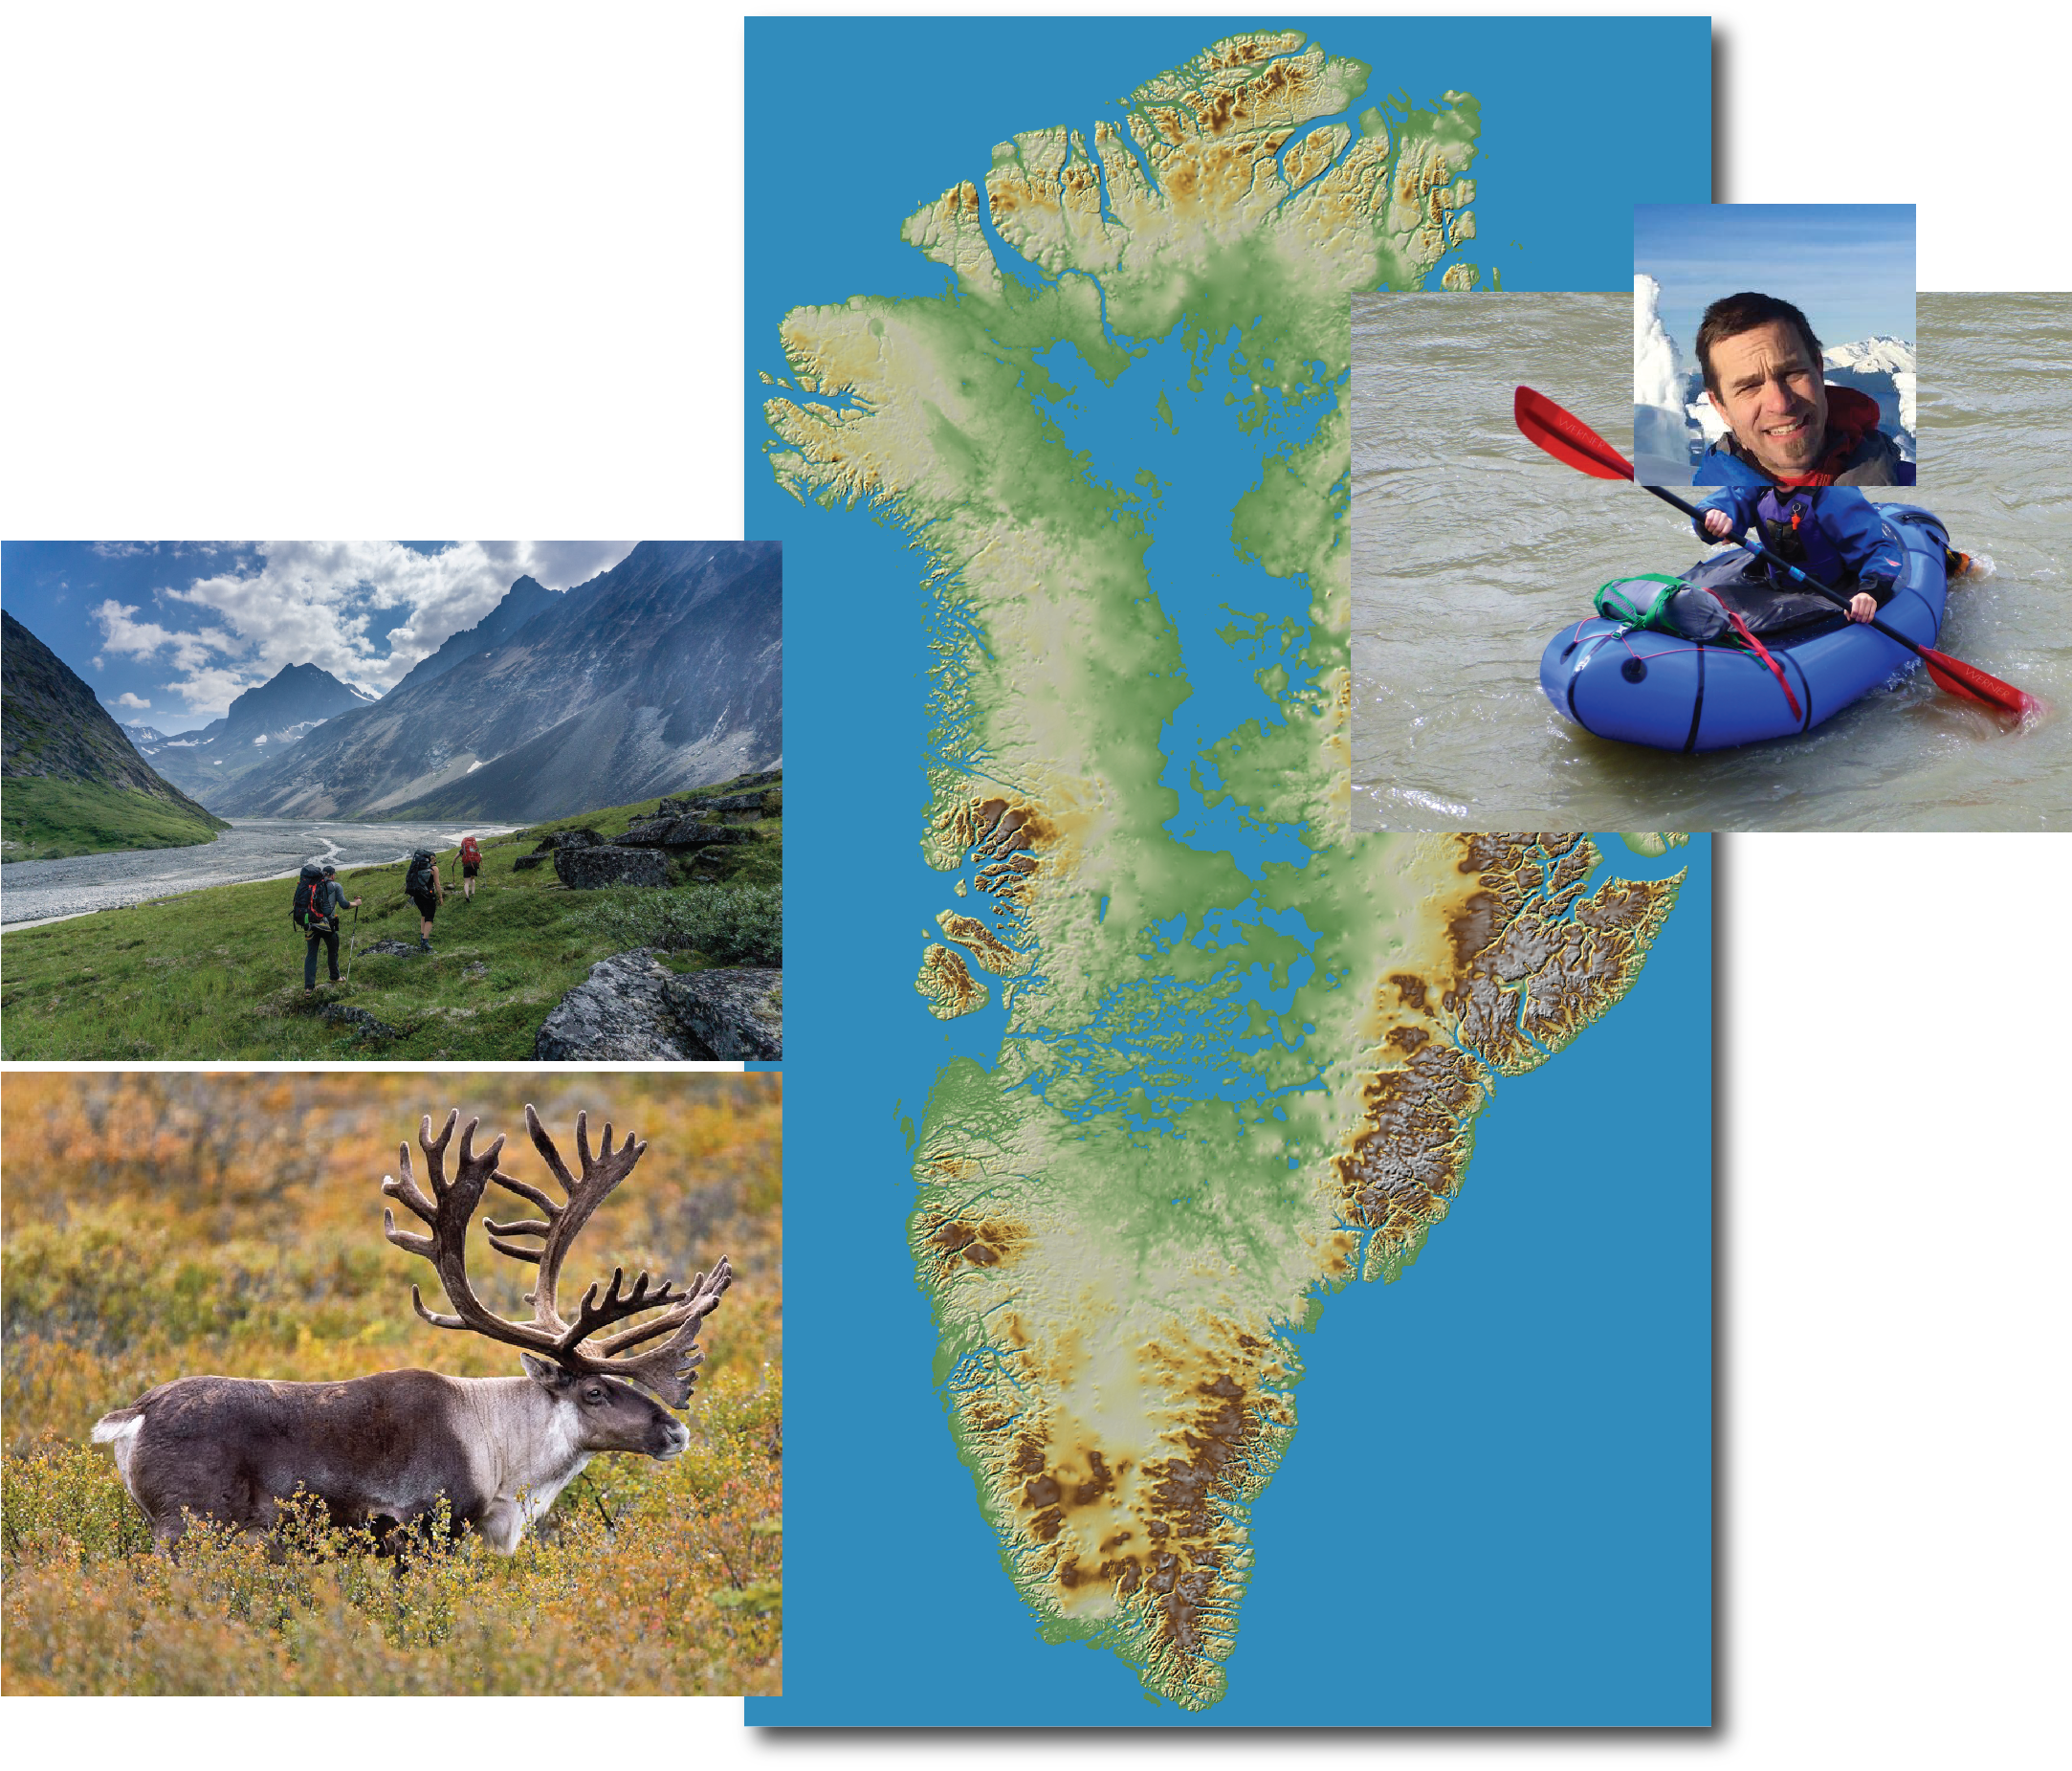
\includegraphics[height=\paperheight,width=\paperwidth]{gris-green-collage-all}};}
} 


\begin{frame}[plain]
\end{frame}

\end{document}